%%%%%%%%%%%%%%%%%%%%%%%%%%%%%%%%%%%%%%%%%
% Journal Article
% LaTeX Template
% Version 1.4 (15/5/16)
%
% This template has been downloaded from:
% http://www.LaTeXTemplates.com
%
% Original author:
% Frits Wenneker (http://www.howtotex.com) with extensive modifications by
% Vel (vel@LaTeXTemplates.com)
%
% License:
% CC BY-NC-SA 3.0 (http://creativecommons.org/licenses/by-nc-sa/3.0/)
%
%%%%%%%%%%%%%%%%%%%%%%%%%%%%%%%%%%%%%%%%%

%----------------------------------------------------------------------------------------
%	PACKAGES AND OTHER DOCUMENT CONFIGURATIONS
%----------------------------------------------------------------------------------------

\documentclass[]{article}

\usepackage{blindtext} % Package to generate dummy text throughout this template 

\usepackage[sc]{mathpazo} % Use the Palatino font
\usepackage[T1]{fontenc} % Use 8-bit encoding that has 256 glyphs
\linespread{1.05} % Line spacing - Palatino needs more space between lines


\usepackage[english]{babel} % Language hyphenation and typographical rules

\usepackage[hmarginratio=1:1,top=15mm,left= 10mm, right=10mm, bottom= 8mm]{geometry} % Document margins
\usepackage[hang, small,labelfont=bf,up,textfont=it,up]{caption} % Custom captions under/above floats in tables or figures
\usepackage{booktabs} % Horizontal rules in tables

\usepackage{lettrine} % The lettrine is the first enlarged letter at the beginning of the text

\usepackage{enumitem} % Customized lists
\setlist[itemize]{noitemsep} % Make itemize lists more compact
\usepackage[dvips]{graphicx}
\graphicspath{{noiseimages/}}
\usepackage{listings}
\usepackage{color}
\usepackage{multirow}
\usepackage{longtable}
\usepackage{xcolor}
\usepackage{hyperref}
\definecolor{linkcolor}{HTML}{799B03} % цвет ссылок
\definecolor{urlcolor}{HTML}{799B03} % цвет гиперссылок

\hypersetup{pdfstartview=FitH,  linkcolor=linkcolor,urlcolor=urlcolor, colorlinks=true}



% Define Language
\lstdefinelanguage{Protobuf}
{
	% list of keywords
	morekeywords={
		int32,
		message,
		enum,
		double,
		string,
		required
	},
	sensitive=false, % keywords are not case-sensitive
	morecomment=[l]{//}, % l is for line comment
	morecomment=[s]{/*}{*/}, % s is for start and end delimiter
	morestring=[b]" % defines that strings are enclosed in double quotes
}

\usepackage{abstract} % Allows abstract customization
\renewcommand{\abstractnamefont}{\normalfont\bfseries} % Set the "Abstract" text to bold
\renewcommand{\abstracttextfont}{\normalfont\small\itshape} % Set the abstract itself to small italic text

\usepackage{titlesec} % Allows customization of titles
%\renewcommand\thesection{\Roman{section}} % Roman numerals for the sections
%\renewcommand\thesubsection{\roman{section}} % roman numerals for subsections
\titleformat{\section}[block]{\large\scshape}{\thesection.}{1em}{} % Change the look of the section titles
%\titleformat{\subsection}[block]{\large}{\thesubsection.}{1em}{} % Change the look of the section titles

%\usepackage{fancyhdr} % Headers and footers
%\pagestyle{fancy} % All pages have headers and footers
%\fancyhead{} % Blank out the default header
%\fancyfoot{} % Blank out the default footer
% Custom header text
%\fancyfoot[RO,LE]{\thepage} % Custom footer text
\pagestyle{empty} 

\usepackage{titling} % Customizing the title section

\usepackage{hyperref} % For hyperlinks in the PDF

%----------------------------------------------------------------------------------------
%	TITLE SECTION
%----------------------------------------------------------------------------------------

\setlength{\droptitle}{-3\baselineskip} % Move the title up

\pretitle{\begin{center}\huge\bfseries} % Article title formatting
\posttitle{\end{center}} % Article title closing formatting
\title{Telemetry for getting statistics for which features are used the most in Krita} % Article title

\begin{document}
%\date{}
\maketitle
\section{Contact Information}
\textbf{Full name:}~~~~~~~~~~~~~~~~~Alexey Kapustin \\
\textbf{Email:}~~~~~~~~~~~~~~~~~~~~~~~~djkah11@yandex.com \\
\textbf{IRC nickname:      }~~~~~~~~~akap \\
\textbf{Telegram nickname: }~aluka1 \\
\textbf{Phone: }~~~~~~~~~~~~~~~~~~~~~~8-999-986-73-81 \\
\textbf{Location:          }~~~~~~~~~~~~~~~~~~Moscow, Russia
\section{Problem}
Krita contains a large number of tools for painters, a large number of settings and features.
Their number increases every year, but not all of them are popular. More precisely, the critics want to know which of the options are popular. Based on this information, you can determine the vector of further work, finalize popular, but not too well-implemented features, remove old, useless functions.
The collection of statistics will help to create  achievements to the Steam. Achievements for Krita is good marketing solution, which help us to find new users. It would be reasonable to make two versions: Steam version and non-Steam version.

%\begin{itemize}
%\item Donec dolor arcu, rutrum id molestie in, viverra sed diam
%\item Curabitur feugiat
%\item turpis sed auctor facilisis
%\item arcu eros accumsan lorem, at posuere mi diam sit amet tortor
%\item Fusce fermentum, mi sit amet euismod rutrum
%\item sem lorem molestie diam, iaculis aliquet sapien tortor non nisi
%\item Pellentesque bibendum pretium aliquet
%\end{itemize}
%\blindtext % Dummy text
%Text requiring further explanation\footnote{Example %footnote}.
\section{Implementation}
\subsection{Client-side}
The main idea is to use Google Protobuf logs to write out necessary information. All information is stored in the logs and as necessary (too large log file, not sent for a long time, etc.) is sent to the server. Sending in the original form the information is irrational, so before sending, the information from the log is analyzed and only the "squeeze" from this information is sent to the server.\\
Main data that we want to analyze:




%\centering
\begin{longtable}{|c|c|l|}
\hline
Information about & Source & Data \\
\hline \hline

Tools & \begin{tabular}[x]{@{}c@{}}KisTool::activate, KisTool:deactivate,\\etc, overloaded in specific tools\end{tabular}
 &\begin{lstlisting}[language=Protobuf]
int32 activationTime;
int32 useTime;
int32 kindTool;
\end{lstlisting} \\
\hline \hline
Strokes & \begin{tabular}[x]{@{}c@{}} KisToolFreehandHelper::initPaintImpl\\ KisToolFreehandHelper::endPaint etc\end{tabular}
&  \begin{lstlisting}[language=Protobuf]
int32 distance;
int32 time;
int32 opacity;
string currentFgColor;
FillStyle fillStyle;
StrokeStyle strokeStyle;
\end{lstlisting}\\
\hline \hline
Presets & KisToolFreehandHelper::initPaintImpl &
    \begin{lstlisting}[language=Protobuf,escapechar=|]
string koid;
OutlineMode outlinemode;
double paintOpFlow;
string compositeMode;
double  savedBrushSize;
int32  hashCode;[|\ref{fml1}|]
	\end{lstlisting} \\
	\hline \hline
	Actions & KisMainWindows actioncollection() &
	\begin{lstlisting}[language=Protobuf]
string name;
string actionSource;
	\end{lstlisting} \\
	\hline%\hline
	

\end{longtable}
\label{fml1} [3.1]: It is required to save presets into map structure for less size of log.\\

\subsection{Server-side}
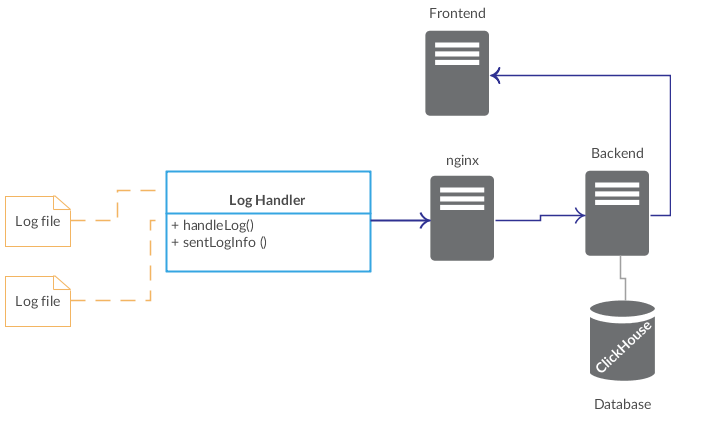
\includegraphics[scale=0.8]{scheme}
\subsubsection{Own stats}
Unfortunately, clickstream services are focused on gathering information from websites. Own implementation allows you to create a convenient api for yourself, and also leaves room for further development and expansion.\\
Scheme description:
The data from the user is serialized and sent to our nginx, which proxy requests to the backend.On the backend, there is deserialization and recording of information in the database.  The information from the database returns to the backend, where it then goes to the front-line. This scheme seems somewhat redundant, but it has an extensible architecture and is capable of withstanding highloads. Nginx is  an optional element, but with increasing load, this architecture will allow you to scale horizontally
\subsubsection{Steam achivments}
It is required to add Steam Sdk.We should to create achievements via Steam web interface. Filling in the list of achievements will be discussed with community. Before any functions can be used, first  {\itshape SteamAPI\_Init()} must be called.After that we can call \textit{SteamUserStats()->SetAchievement( "Draw\_the\_length\_of\_the\_equator") }and set specific achivment.
\subsection{Technologies}
Nginx is widespread server, which is used by nearby 70\% percents of top-100 worldwide side. ClickHouse allows you to perform analytical queries interactively on real-time data. The system is scalable to very large amounts of data. 



\section{Timeline}
Work schedule ~~~~~~~~~~~~~~~~~~~~~~~~~~~~~~~~~~~~~~~~~~~~~~~~~~~~Implementation timeline
	\begin{table}[h]
		\begin{minipage}{.4\textwidth}
			\centering
			\begin{tabular}{|c|c|}
				\hline
				 Period & Work\\
				\hline 22 May -4 June  & End of the school year. Opportunity to work 7-10 hours a week.
				\\
				2,3153 & 1,3644\\
				\hline
			\end{tabular}
		\end{minipage}
		\begin{minipage}{.4\textwidth}
			\centering
			\begin{tabular}{|c|c|}
				\hline Period  & Work\\
				\hline 0,2733 & 5,3763\\
				0,9496 & 5,3763\\
				\hline
			\end{tabular}
		\end{minipage}
	\end{table}
	



%------------------------------------------------




\end{document}
